% Q18：火星探测器轨道示意；椭圆、火星圆及坐标长度均非比例。
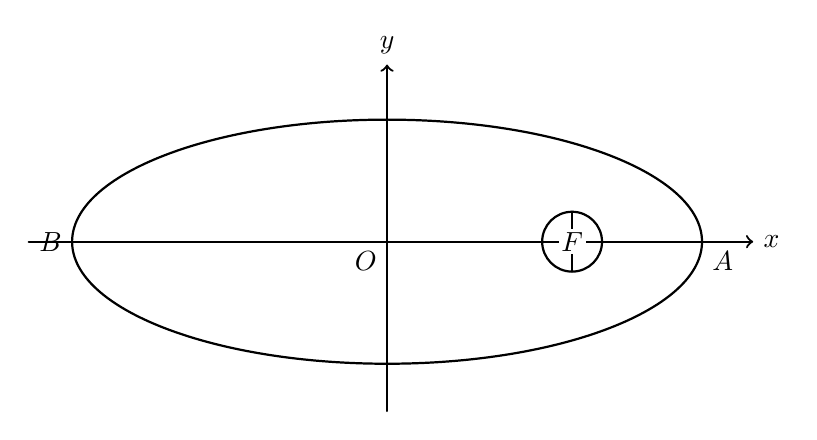
\begin{tikzpicture}[line cap=round,line join=round,thick]
  \coordinate (O) at (0,0);
  \coordinate (B) at (-4,0);
  \coordinate (A) at (4,0);
  \coordinate (F) at (2.35,0);

  \draw[->] (-4.55,0)--(4.65,0) node[right] {$x$};
  \draw[->] (0,-2.15)--(0,2.25) node[above] {$y$};
  \draw (O) ellipse (4 and 1.55);
  \draw (F) circle[radius=0.38];
  \draw (2.35,-0.38)--(2.35,0.38);

  \node[below left] at (O) {$O$};
  \node[left] at (B) {$B$};
  \node[fill=white,inner sep=1pt] at (F) {$F$};
  \node[below right] at (A) {$A$};
\end{tikzpicture}
